\maketitle


\section{Predicting Bike Station Occupancy}
\subsection{Feature Engineering}
\subsubsection{Selection of Station}
In choosing the stations I was going to use I decided to display them on a map.
This would make it easier to choose stations which would have different behaviour.
I decided to choose station 97 (Kilmainham Gaol) as it is the furthest from the city center.
I also chose station 109 (Buckingham Street) as it is beside Connolly and I assumed it would have drastically different behaviour than my other station.

\begin{figure}[H]
\centering
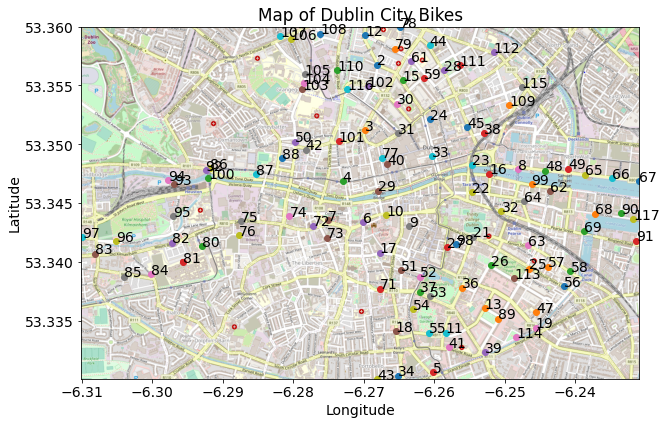
\includegraphics[width=0.5\textwidth]{images/map.png}
\caption{Map of Dublin Bike stations.}
\end{figure}

The data that I needed was the time and number of available bikes.

\begin{figure}[H]
    \centering
    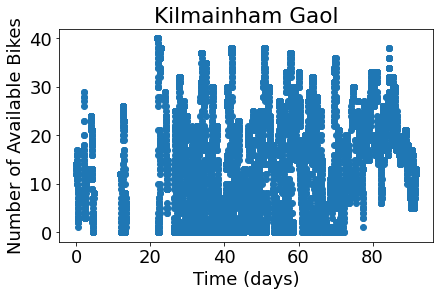
\includegraphics[width=0.5\textwidth]{images/kilmainham data.png}
    \caption{Map of Dublin Bike stations.}
    \end{figure}
\par 

\begin{figure}[H]
    \centering
    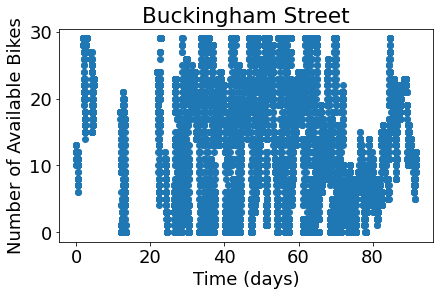
\includegraphics[width=0.5\textwidth]{images/buckingham data.png}
    \caption{Map of Dublin Bike stations.}
    \end{figure}
Much of the data was missing
Interpolating
downsampling

\par 


\subsection{Machine Learning Methodology}
The Machine learning methods I decided to use are\dots
\subsubsection{Method 1}
\subsubsection{Method 2}

\subsection{Evaluation}
